\documentclass[journal,12pt]{IEEEtran} % use the `journal` option for ITherm conference style
\IEEEoverridecommandlockouts
% The preceding line is only needed to identify funding in the first footnote. If that is unneeded, please comment it out.

\usepackage[english]{babel}
\usepackage[utf8x]{inputenc}
\usepackage{amsmath}

\usepackage{graphicx}
\usepackage{float}
\usepackage{caption}
\usepackage{subcaption}
\captionsetup{justification=centering}

\usepackage{url}
\def\UrlBreaks{\do\/\do-}
\usepackage{breakurl}



\begin{document}

\title{Conference Paper Title*}

\author{%%%% author names
    \IEEEauthorblockN{Tziporah Horowitz}% first author
    \\%%%% author affiliations
    \IEEEauthorblockA{Johns Hopkins University, Whiting School of Engineering}\\% first affiliation
    \IEEEauthorblockA{ACM 725 - Theory of Statistics I}
}

\maketitle
\clearpage

\begin{abstract}
    This document is a model and instructions for \LaTeX.
    This and the IEEEtran.cls file define the components of your paper [title, text, heads, etc.]. *CRITICAL: Do Not Use Symbols, Special Characters, Footnotes,
    or Math in Paper Title or Abstract.
\end{abstract}
\clearpage


\section{Introduction}
Statistical binary classification is a process used in medical testing to determine if a patient has a certain disease or not.
It often employs supervised learning to determine decision classes based on predefined rules.
While methods such as decision trees, random forests, and neural networks are commonly used in other applications of binary classification, logistic regression offers medical testing a number of advantages due to its probabilistic nature and its relationship with the odds ratio~\citep{Schober2021-vs}. 
If interpreted correctly, it can provide a measure of associated risk between the independent variables and the binary outcome.

The upcoming sections will provide an overview of the statistical theory behind logistic regression, followed by an analysis of the association between various risk factors and the chances of a patient contracting heart desease. To measure the associated risk, this paper provides a synopsis of four common methods: \emph{risk difference}, \emph{relative risk}, \emph{odds ratio's}, and \emph{marginal effects}.

\section{Logistic Regression}
Logistic regression was proposed as an alternative to ordinary least squares (OLS) regression in the 1960's in the context of predicting binary outcomes~\citep{An-Introduction-to-Logistic-Regression-Analysis-and-Reporting}. 
While OLS relies on linearity, normality, and continuity, logistic regression utilizes the \emph{logit} or log-odds function (eq. \ref{eq:logit}) to predict the probability of an outcome falling into a specific category. 
\begin{align}
    \logit{Y} = \ln \left( \frac{p}{1-p} \right) \label{eq:logit}
\end{align}
Using the logit function allows the modeler to create a sigmoidal relationship between two classes, which appears linear in the middle and curved on the ends.

Let $\hat{p}$ be the probability of an outcome occurring given a specific value of a feature:
\begin{align}
    \hat{p} = \prob{Y = 1 | X = x} = \frac{1}{1 + e^{-(\alpha + \beta x)}} \label{eq:sigmoid}
\end{align}
By rewriting the sigmoid function in equation \ref{eq:sigmoid} and taking its natural logarithm, we can derive a linear relationship between the log-odds of $\hat{p}$ and the feature variable, $x$:
\begin{align*}
    \hat{p} &= \frac{1}{1 + e^{-(\alpha + \beta x)}} \\
    \frac{1}{\hat{p}} &= 1 + e^{-(\alpha + \beta x)} \\
    \frac{1}{\hat{p}} - 1 &= e^{-(\alpha + \beta x)} \\
    \frac{1 - \hat{p}}{\hat{p}} &= e^{-(\alpha + \beta x)} \\
    \ln \left( \frac{1 - \hat{p}}{\hat{p}} \right) &= -(\alpha + \beta x) \\
    \ln \left( \frac{\hat{p}}{1 - \hat{p}} \right) &= \alpha + \beta x
\end{align*}
Thus, logistic regression can be expressed a generalized linear model (GLM), such that
\begin{align*}
    \logit{Y} = \vec{\beta}\matrx{X}
\end{align*}
where $\vec{\beta}$ is the vector of regression coefficients and $\matrx{X}$ is the matrix of feature variables.

While there are a number of different techniques, the regression coefficients are typically estimated using the \emph{maximum likelihood} method. The maximum likelihood method aims to maximize the likelihood of reproducing the data given the parameter estimates~\citep{An-Introduction-to-Logistic-Regression-Analysis-and-Reporting}. Let $Y_i | X_i \stackrel{ind}{\sim} \bern{f(\vec{x}_i)}$. Then, the joint likelihood function is:
\begin{align*}
    \likelihood{\vec{\beta}} =
    \prob{Y_1 = y_1, \dots, Y_n = y_n | \vec{x_1}, \dots, \vec{x_n}}
    = \prod_{i=1}^n f(\vec{x}_i)^{y_i} \left( 1 - f(\vec{x}_i) \right)^{1-y_i}
\end{align*}
Thus, the maximum likelihood estimate of the logistic regression function is:
\begin{align}
    \vec{\beta} = \argmax{\vec{w}}{\prod_{i=1}^n \left( \frac{1}{1+e^{-\vec{w}\matrx{X}}} \right)^{y_i} \left( \frac{1}{1+e^{\vec{w}\matrx{X}}} \right)^{1-y_i} \label{eq:mle}}
\end{align}
However, it is important to note that the gradient vector of equation \ref{eq:mle} cannot be solved for zero, and therefore has no closed form.
A common approach for solving equation \ref{eq:mle} numerically is the \emph{reweighted least squares} algorithm~\citep{Wasserman2004}.

The coefficients of a logistic regression model can be interpreted as, $\beta_i$ is the change of the log-odds of the target occurring per one unit increase of $X_i$ when all other variables $X_j$ $(j \neq i)$ are fixed. 
The estimates, $\hat{\beta}_i$ can be tested for statistical significance using a Wald test where
\begin{align*}
    H_0&: \hat{\beta}_i = 0 \\
    H_1&: \hat{\beta}_i \neq 0
\end{align*}
If $\norm{W} = \norm{\frac{\hat{\beta}_i - 0}{\hat{\text{se}}}}$ is greater than $z_{\frac{\alpha}{2}}$, then the null-hypothesis is rejected and $\hat{\beta}_i$ is considered statistically significant.
 
\clearpage

\section{Methods}
\begin{table}[b]
    \caption{Contingency Matrix}\label{table:contingency}
    \centering
    \begin{tabular}{|r|cc|}
        \hline & {\text{ Diseased }} & {\text{ Healthy }} \\
        \hline {\text{ Exposed }} & $D_E$ & $H_E$ \\
        {\text{ Unexposed }} & $D_U$ & $H_U$ \\ \hline
    \end{tabular}
\end{table}

There are several ways to measure the association between a risk factor and the binary outcome of contracting a disease.
The following sections discuss the four approaches used in this analysis to determine the associated risk of various factors in the context of patients contracting heart disease.
Sections \ref{subsec:associated-risk-difference} through \ref{subsec:odds-ratio} refer to table~\ref{table:contingency} for simplification.


\subsection{Risk Difference}\label{subsec:associated-risk-difference}

Often considered the simplest approach for measuring associated risk, \emph{risk difference} or \emph{absolute risk difference} (ARD) is the difference in the outcome rates between patients with the risk factor and patients without the risk factor~\citep{Statistical-hypothesis-testing}.
Using the matrix in~\ref{table:contingency}, risk difference can be defined mathematically as:
\begin{align*}
 \text{ARD} = \ARD{D_{E}}{H_{E}}{D_{U}}{H_{U}}
\end{align*}
While the risk difference is easy to compute, its interpretation is often misleading and can only explain the associated risk between a single factor and the target.

\subsection{Relative Risk}\label{subsec:relative-risk}
Similar to risk difference, \emph{relative risk} compares the outcome rates between patients with the risk factor and patients without the risk factor.
However, relative risk is computed as a ratio (RR) rather than a difference~\citep{Statistical-hypothesis-testing}.
The risk ratio is defined as:
\begin{align*}
 \text{RR} = \RR{D_{E}}{H_{E}}{D_{U}}{H_{U}}
\end{align*}
Relative risk is a useful statistic because it quantifies the probability of a patient with exposure contracting the disease relative to a patient without exposure.
Risk ratios that are close to $1$ indicate that the risk of contracting the disease for an exposed patient is the same as the risk for an unexposed patient.
In contrast, risk ratios that are far from $1$ indicate that there is an association between the variables.
This allows one to create a confidence interval using the hypothesis test,
\begin{align*}
    H_0&: RR = 1 \\
    H_1&: RR \neq 1
\end{align*}
The risk ratio is considered a valid measure of relative risk for studies in which the sampling is dependent on the exposure of interest such as, randomized controlled trials or cohort and cross-sectional studies~\citep{Relative-Measures-of-Association-for-Binary-Outcomes}.
Like risk difference, relative risk can only explain the associated risk between a single factor and the target.


\subsection{Odds Ratio}\label{subsec:odds-ratio}
Often confused with risk ratio, \emph{odds ratio} compares the statistical odds of the outcome in the exposed group to that of the outcome of the unexposed group.
It is defined mathematically as:
\begin{align*}
 \text{OR} = \OR{D_{E}}{H_{E}}{D_{U}}{H_{U}}
\end{align*}
Like the risk ratio, odds ratios that are close to $1$ indicate no association between exposure and contracting the disease, and odds ratios that are far from $1$ indicate that there is an association between the variables.
One can also create a confidence interval for the odds ratio using a similar hypothesis test to that of the risk ratio, such that
\begin{align*}
    H_0&: OR = 1 \\
    H_1&: OR \neq 1
\end{align*}
While the odds ratio is typically considered the \enquote{only valid measure of relative association in traditional case-control studies}~\citep{Relative-Measures-of-Association-for-Binary-Outcomes}, it is frequently misinterpreted as the risk ratio.
However, in cases where the risk factor is relatively small ($< 10 \%$), the odds ratio approximates the risk ratio:
\begin{align*}
%    \begin{matrix}
%        \Lim{D_E}{0}{D_E + H_E} = H_E \\
%        \Lim{D_U}{0}{D_U + H_U} = H_U
%    \end{matrix} &\implies
    \RR{D_{E}}{H_{E}}{D_{U}}{H_{U}} \approx \OR{D_{E}}{H_{E}}{D_{U}}{H_{U}}
\end{align*}
if $D_E$ and $D_U$ are small.

The odds ratio can be applied in multi-parameter settings when computed in a logistic regression analysis, due to its inherent calculation of the logit (or log-odds) function.
To obtain the odds ratio of a logistic regression model, one simply has to exponentiate the coefficients.


\subsection{Marginal Effects}\label{subsec:marginal-effects}

A \emph{marginal effect} (or incremental effect) is the change in the probability that an outcome occurs as the risk factor changes by one unit.
It is often used in logistic regression analysis and other GLM's to explain the incremental risk associated with each factor~\citep{Marginal-Effects—Quantifying-the-Effect-of-Changes-in-Risk-Factors-in-Logistic-Regression-Models}.
Marginal effects are determined by taking the partial derivative of the regression equation with respect to each variable.
They are simpler to interpret than odds ratios and are easier to compare across different studies.
There are many ways to represent the marginal effect for a sample, the most common of which is the \emph{average marginal effect} across all patients in the dataset.

\subsection{The Analysis}\label{subsec:analysis}

For this analysis, the \emph{Heart Disease Dataset} was collected from kaggle.com~\citep{Heart-disease-dataset}.
The dataset includes data that was compiled from four databases in 1988 and consists of 1025 rows and 14 columns: 13 predictors and 1 target.
The predictors include 5 continuous variables: age, resting blood pressure, serum cholestoral (in mg/dl), maximum heart rate achieved, and ST depression induced by exercise relative to rest (oldpeak);
and 8 categorical variables: sex, chest pain type, fasting blood sugar $>$ 120 mg/dl (true or false), resting electrocardiographic results, exercise induced angina (yes or no), the slope of the peak exercise ST segment, number of major vessels (0-3) colored by flourosopy, and thal (normal, fixed defect, reversible defect).
Figure~\ref{fig:skim} shows the \emph{skimpy} summary of all 14 variables and figure~\ref{fig:subdistributions} shows the distributions of predictor variables when compared to the target, a binary indicator for the patient having heart disease.

\begin{figure*}[tp]
    \centering
    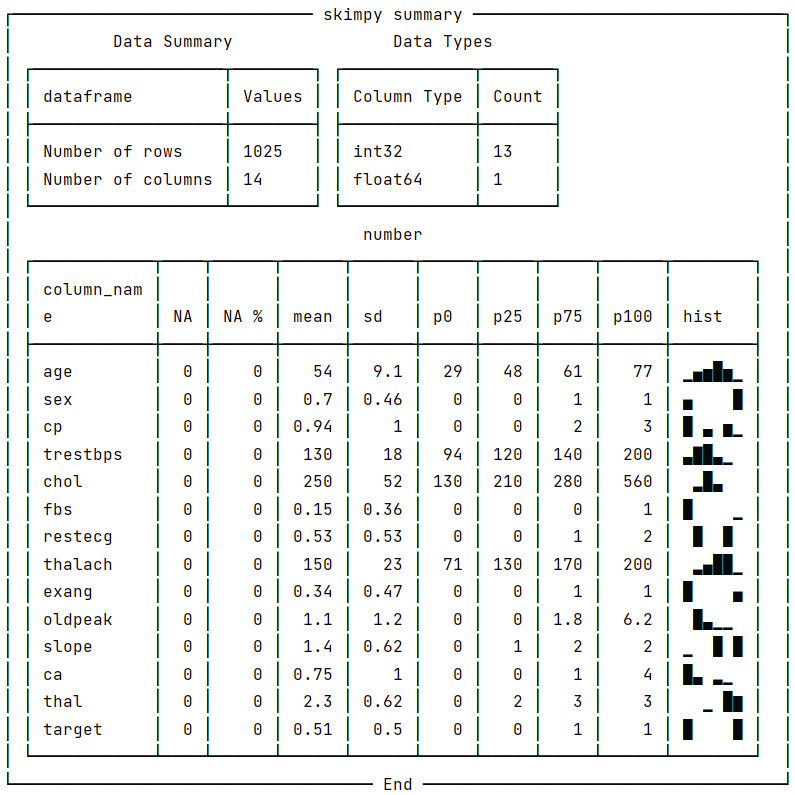
\includegraphics[width=.7\textwidth]{plots/skimpy-summary.png}
     \caption[Figure]{Summary of Variables} \label{fig:skim}
\end{figure*}

\begin{figure*}[btp]
     \centering
     \begin{subfigure}[b]{0.32\textwidth}
         \centering
         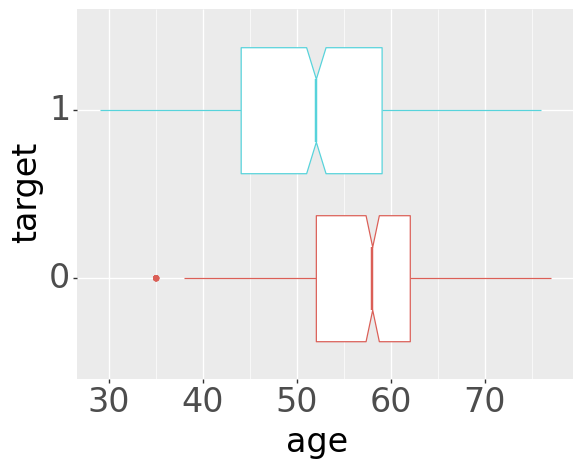
\includegraphics[width=\textwidth]{plots/target-age}
     \end{subfigure}
     \begin{subfigure}[b]{0.32\textwidth}
         \centering
         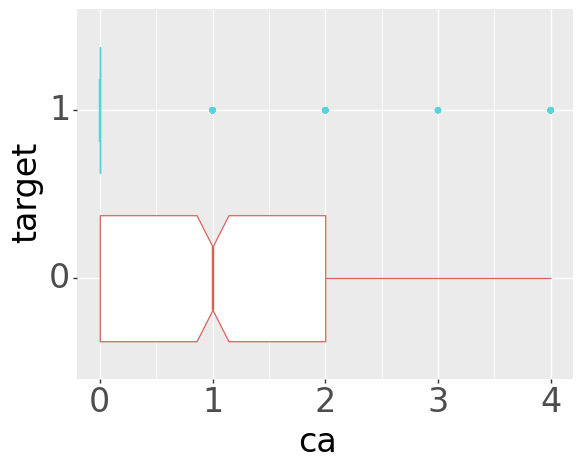
\includegraphics[width=\textwidth]{plots/target-ca}
     \end{subfigure}
     \begin{subfigure}[b]{0.32\textwidth}
         \centering
         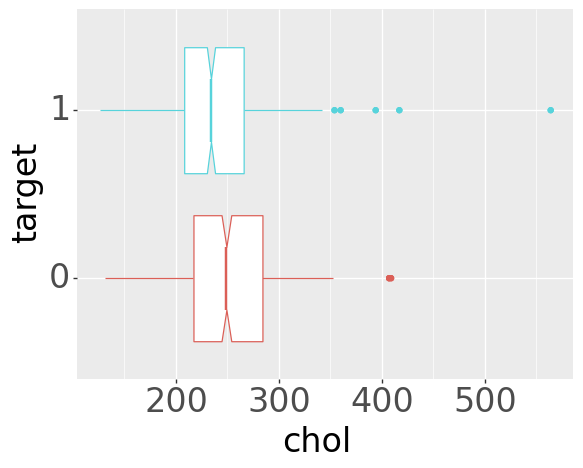
\includegraphics[width=\textwidth]{plots/target-chol}
     \end{subfigure}

     \begin{subfigure}[b]{0.32\textwidth}
         \centering
         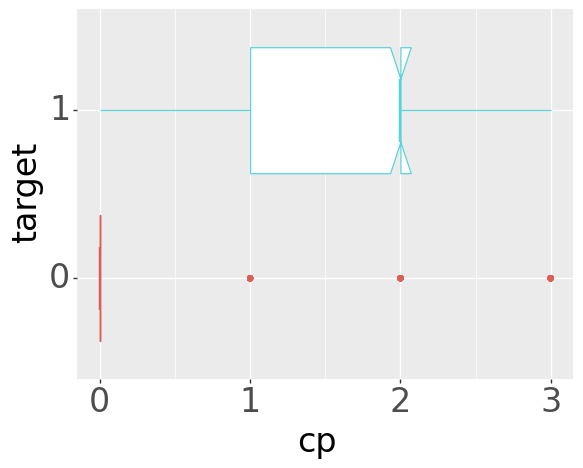
\includegraphics[width=\textwidth]{plots/target-cp}
     \end{subfigure}
     \begin{subfigure}[b]{0.32\textwidth}
         \centering
         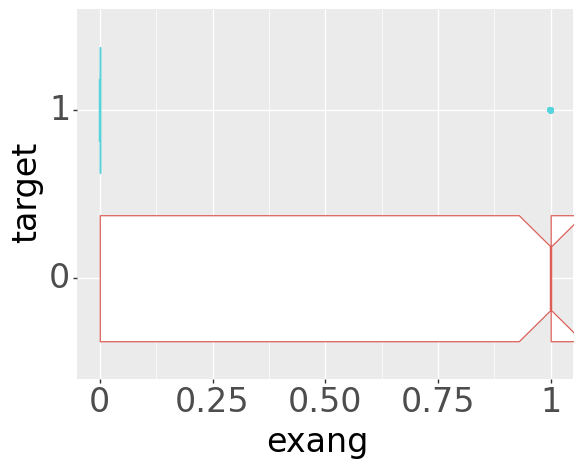
\includegraphics[width=\textwidth]{plots/target-exang}
     \end{subfigure}
     \begin{subfigure}[b]{0.32\textwidth}
         \centering
         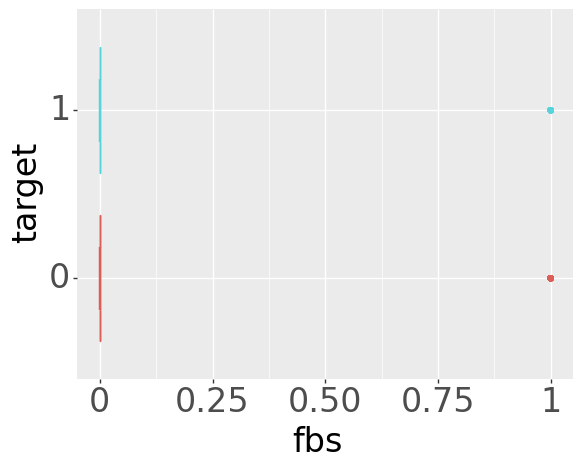
\includegraphics[width=\textwidth]{plots/target-fbs}
     \end{subfigure}

     \begin{subfigure}[b]{0.32\textwidth}
         \centering
         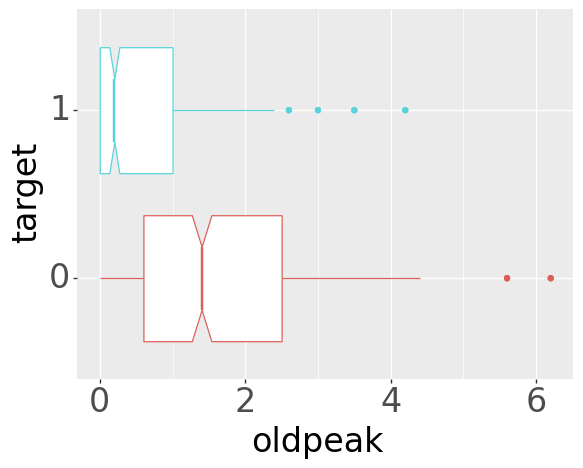
\includegraphics[width=\textwidth]{plots/target-oldpeak}
     \end{subfigure}
     \begin{subfigure}[b]{0.32\textwidth}
         \centering
         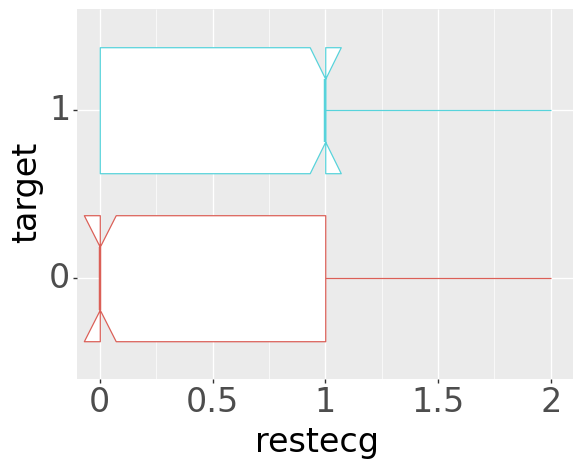
\includegraphics[width=\textwidth]{plots/target-restecg}
     \end{subfigure}
     \begin{subfigure}[b]{0.32\textwidth}
         \centering
         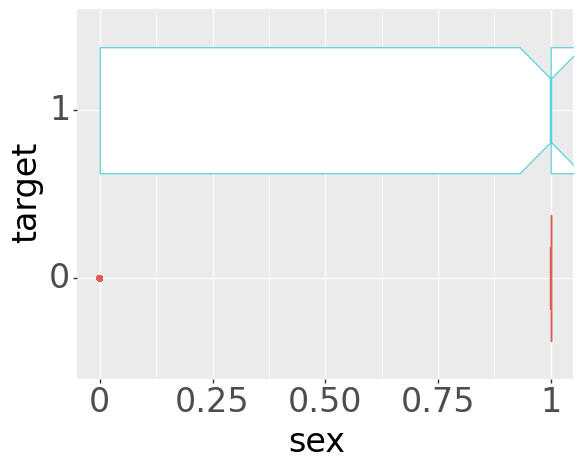
\includegraphics[width=\textwidth]{plots/target-sex}
     \end{subfigure}

     \begin{subfigure}[b]{0.32\textwidth}
         \centering
         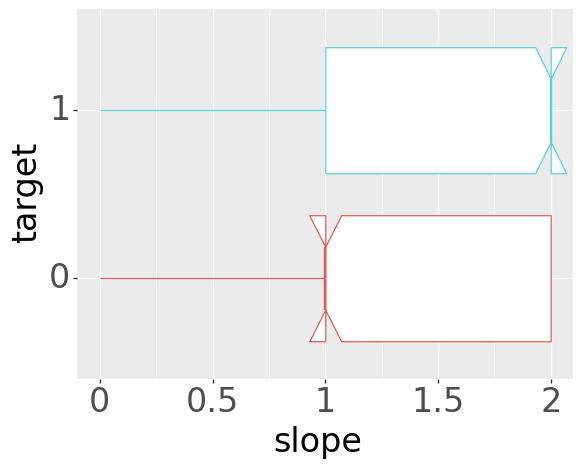
\includegraphics[width=\textwidth]{plots/target-slope}
     \end{subfigure}
     \begin{subfigure}[b]{0.32\textwidth}
         \centering
         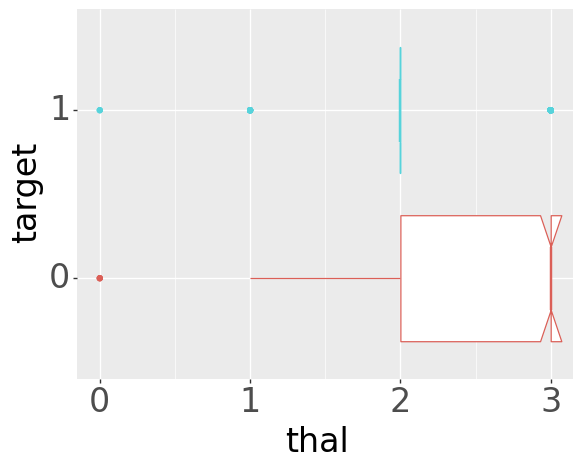
\includegraphics[width=\textwidth]{plots/target-thal}
     \end{subfigure}
     \begin{subfigure}[b]{0.32\textwidth}
         \centering
         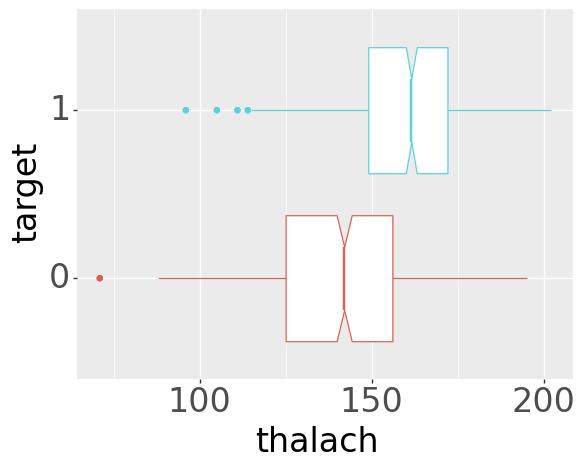
\includegraphics[width=\textwidth]{plots/target-thalach}
     \end{subfigure}

     \begin{subfigure}[b]{0.32\textwidth}
         \centering
         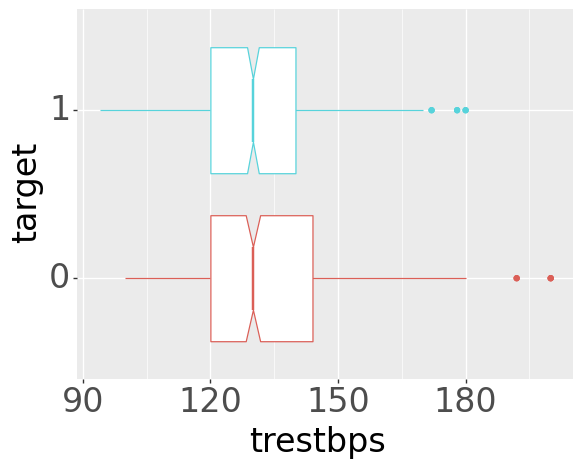
\includegraphics[width=\textwidth]{plots/target-trestbps}
     \end{subfigure}

     \caption[Figure]{Distributions of Feature Variables} \label{fig:subdistributions}
\end{figure*}

Prior to computing any of the above measures of associated risk, the data was imported into Python (3.9) using \inlinecodettt{pandas} and dummy variables were created for the categorical columns.
Individual risk differences and risk ratios were then computed for each predictor variable.
The dataset was then divided into a $3:2$ train-test split so that a logistic regression model can be fit.
Two models were fit using the training set to the objective function,
\begin{align*}
    p = \boldsymbol{\beta X}
\end{align*}
via \inlinecodettt{statsmodels}.
One was computed with the odds ratio, and the other with marginal effects.
The models were then tested with the remainder of the data and scored using \inlinecodettt{sklearn}.



\section{Results}
\begin{adjustbox}{max width=\textwidth}
    \centering
    \begin{table*}[!bp]
    \caption{Risk Difference and Risk Ratio of Binary Variables} 
    \label{tab:risk}
    \colorbox{gray!20}{
    \resizebox{\textwidth}{!}{
        \begin{tabular}{lrrr}
        \toprule
        {} & Risk Difference & Risk Ratio & RR 95\% Confidence Interval \\
        \midrule
        age                               &         -0.2892 &     0.5671 &          (0.5008, 0.6423)^* \\
        sex                               &         -0.3036 &     0.5809 &          (0.5204, 0.6484)^* \\
        resting blood pressure $>$ 130      &         -0.0888 &      0.839 &          (0.7411, 0.9499)^* \\
        serum cholestoral $>$ 250 ml/dl     &         -0.1512 &     0.7374 &          (0.6473, 0.8401)^* \\
        fasting blood sugar $>$ 120 mg/dl   &         -0.0577 &     0.8893 &           (0.7415, 1.0666) \\
        maximum heart rate achieved $>$ 150 &          0.4067 &      2.364 &          (2.0403, 2.7391)^* \\
        exercise induced angina           &         -0.4633 &     0.3076 &          (0.2483, 0.3809)^* \\
        oldpeak                           &         -0.3773 &      0.435 &          (0.3708, 0.5103)^* \\
        chest pain = 1                    &          0.3455 &     1.7563 &          (1.5815, 1.9503)^* \\
        chest pain = 2                    &          0.3568 &     1.8613 &          (1.6732, 2.0704)^* \\
        chest pain = 3                    &          0.1613 &     1.3219 &          (1.1134, 1.5694)^* \\
        resting electrocardiograph = 1    &          0.1785 &     1.4212 &          (1.2566, 1.6073)^* \\
        resting electrocardiograph = 2    &         -0.3178 &     0.3862 &           (0.1401, 1.0646) \\
        slope = 1                         &         -0.3499 &     0.4837 &          (0.4203, 0.5566)^* \\
        slope = 2                         &          0.3904 &      2.167 &          (1.9032, 2.4674)^* \\
        major vessels colored = 1         &         -0.2837 &     0.5073 &          (0.4105, 0.6268)^* \\
        major vessels colored = 2         &         -0.4101 &     0.2765 &          (0.1859, 0.4112)^* \\
        major vessels colored = 3         &         -0.4104 &     0.2412 &          (0.1308, 0.4448)^* \\
        major vessels colored = 4         &          0.3259 &     1.6422 &           (1.324, 2.0369)^* \\
        thal = 1                          &         -0.1974 &     0.6244 &          (0.4375, 0.8911)^* \\
        thal = 2                          &          0.5203 &     3.1955 &          (2.7033, 3.7772)^* \\
        thal = 3                          &         -0.4894 &     0.3096 &          (0.2562, 0.3742)^* \\
        \bottomrule
        \end{tabular}
    }}
\end{table*}
\end{adjustbox}


\clearpage

\singlespacing
\bibliography{main}
\bibliographystyle{IEEEtran}

\clearpage
\onecolumn

\appendix
\renewcommand{\thesection}{\Alph{section}}

\section{Code}\label{sec:code}

\subsection{data\_summary.py}\label{subsec:data_summary.py}
\lstinputlisting[language=Python,label={lst:summary}]{data_summary.py}

\clearpage

\subsection{associated\_risk.py}\label{subsec:associated_risk.py}
\lstinputlisting[language=Python,label={lst:risk}]{associated_risk.py}

\clearpage

\subsection{models.py}\label{subsec:models.py}
\lstinputlisting[language=Python,label={lst:analysis}]{models.py}


\end{document}
